\documentclass{article}
\usepackage[T1]{fontenc}
\usepackage{lmodern}
\usepackage{graphicx}
\usepackage{amsmath,amssymb}
\usepackage[a4paper,margin=2cm]{geometry}
\usepackage[absolute,overlay]{textpos}
\setlength{\TPHorizModule}{1mm}
\setlength{\TPVertModule}{1mm}
\usepackage[indonesian]{babel}
\usepackage{hyperref}
\setlength{\emergencystretch}{2em}
% unit: Halaman 4

\begin{document}

% === Halaman 4 (llm) ===

\vspace{181.17mm}

\begin{itemize}
    \item Catat bahwa DES adalah sebah standard, sedangkan algoritmanya sendiri bernama DEA (\textit{Data Encryption Algorithm}). Kedua nama ini sering dikacaukan.
    \item DES termasuk ke dalam algoritma kriptografi kunci-simetri dan tergolong ke dalam \textit{cipher} blok.
    \item DES beroperasi pada ukuran blok plainteks 64 bit.
    \item Panjang kunci ekternal = 64 bit (sesuai ukuran blok), tetapi hanya 56 bit yang dipakai (8 bit \textit{parity} tidak digunakan). Bit parity = bit ke-8, 16, 24, dst.
\end{itemize}

% deskripsi: Gambar sampul dokumen FIPS PUB 46 berjudul 'DATA ENCRYPTION STANDARD'
% bbox normalisasi: [0.6800, 0.1600, 0.9400, 0.7700]
\begin{textblock*}{54.60mm}(142.80mm,47.52mm)
\noindent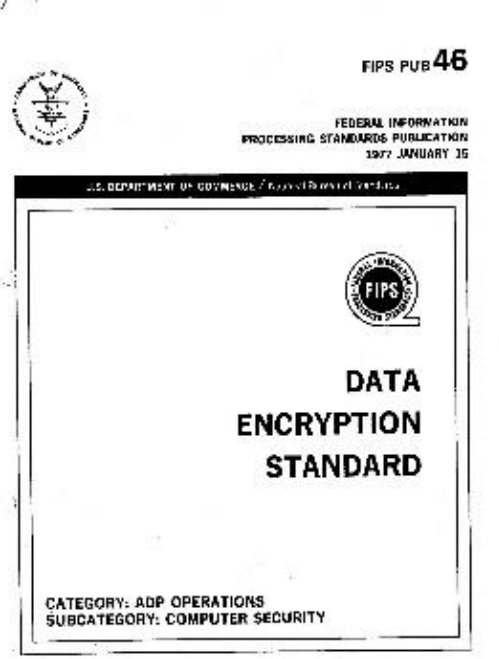
\includegraphics[width=54.60mm,height=181.17mm]{../../images/llm/page_004_img_01.png}%
\end{textblock*}

\end{document}
